\chapter{Experiments}~\label{chap:experiments}

In this chapter we demonstrate performance and comparable results of the proposed Object SLAM system with state of the art online and offline reconstruction systems in terms of trajectory accuracy and object reconstruction quality. We evaluate on the RGBD scenes V2 dataset~\cite{laiUnsupervisedFeatureLearning2014} and the TUM RGBD dataset~\cite{sturmBenchmarkEvaluationRGBD2012}, both of which are established RGBD SLAM benchmarks and compare against baseline methods.

\section{Architecture and Experimental Setup}


To support relatively high frame rate operation in the presence of slow/non-realtime deep learning components our pipeline is highly parallelized. Our system adopts the \textit{Actor} framework, where each component runs asynchronously, and communicates via thread-safe queues.

We implement the semantic segmentation pipeline as a separate python process which serializes the outputs using \texttt{protobuf} and communicates with the client thread via \texttt{zeromq} sockets in the Object SLAM pipeline. Since, instance segmentation is carried out only for keyframes, the asynchronous python process exits early (typically) freeing GPU memory, that can be used for large reconstructions.

I implement the GPU code in CUDA, and leverage the Open3D GPU framework~\cite{dongGPUAcceleratedRobust2019}. In particular, we build on the (in-house) spatially hashed TSDF implementation, implement an additional frame-to-model tracking module, and also build a back-end module for pose graph optimization. We use the optimized spherical ray-casting method to improve performance.

Our experiments were run on a Linux system (Ubuntu 18.04) with Intel i7-6700 CPU at 4.00 GHz and 32GB of RAM and a NVIDIA GTX1080 with 8GB of GPU memory.

\section{Qualitative results}

We first demonstrate qualitative reconstruction results on the RGBD scenes V2 dataset.  Fig.~\ref{fig:rgbd_scene13} shows the object mesh extracted from our scalable volumes with a foreground count threshold. We can see that small objects are clearly reconstructed with details, and the background is correctly filtered.

At a larger scale, Fig.~\ref{fig:objectsandscene} segments teddy bear and computers from the cluttered scene and ensures a low-drift of the trajectory. Fig.~\ref{fig:rgbd_scene12} compares reconstructions from \textit{MaskFusion} \cite{runz_maskfusion_2018} and our system for a given sequence. It can be seen that the object-level reconstruction -- specifically for the cap and sofa -- is much cleaner in our system than in \textit{MaskFusion}.

\begin{figure}[t!]
    \centering
    \subfloat{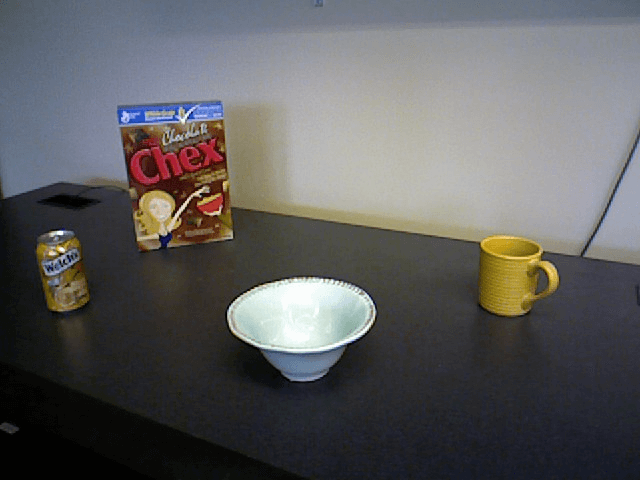
\includegraphics[width=0.5\linewidth]{figs/frame-000218.color.png}}
    \subfloat{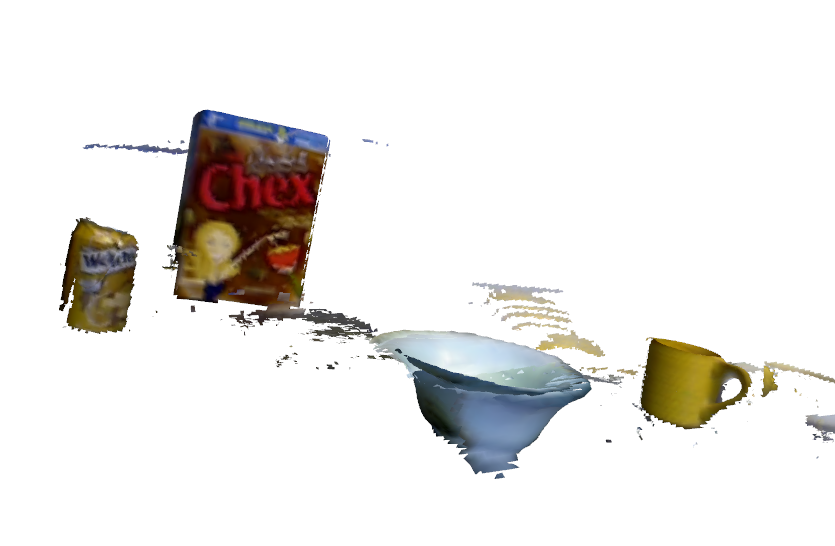
\includegraphics[width=0.5\linewidth]{figs/scene13-objectsonly.png}}
    \caption{Qualitative foreground object reconstruction results on \emph{RGB-D Scene 13} sequence.}
    \vspace*{-1em}
    \label{fig:rgbd_scene13}
\end{figure}

\begin{figure*}[t!]
    \centering
    \subfloat{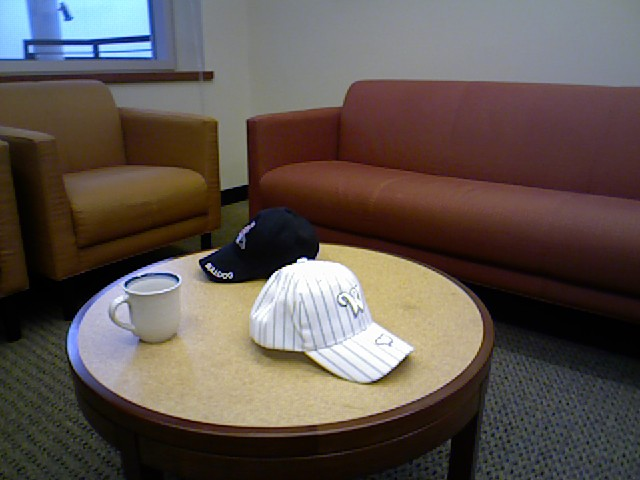
\includegraphics[align=c,width=0.49\linewidth]{figs/frame-000293.color.png}}
    \subfloat{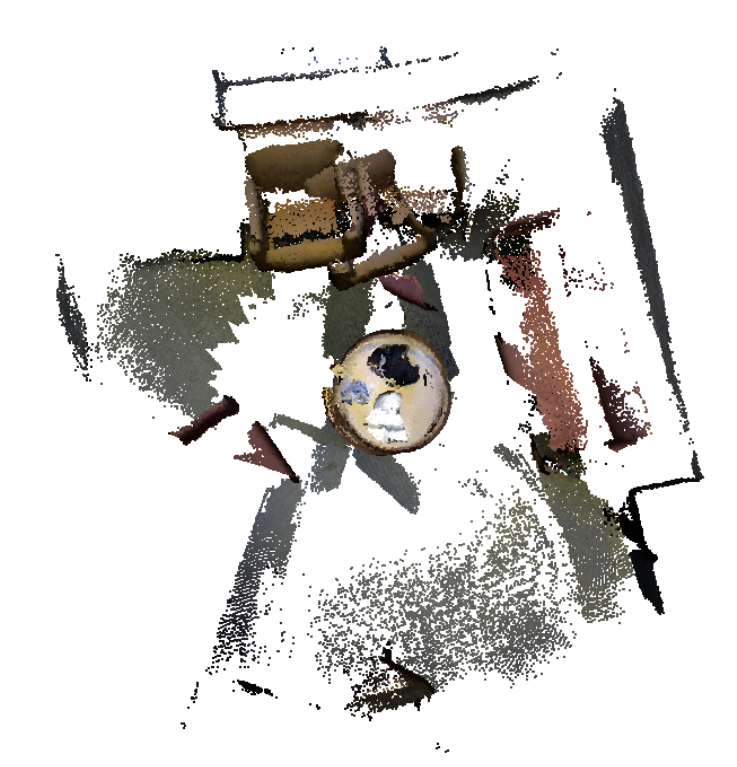
\includegraphics[align=c,width=0.49\linewidth]{figs/mask-fusion-scene12.png}}\\
    \subfloat{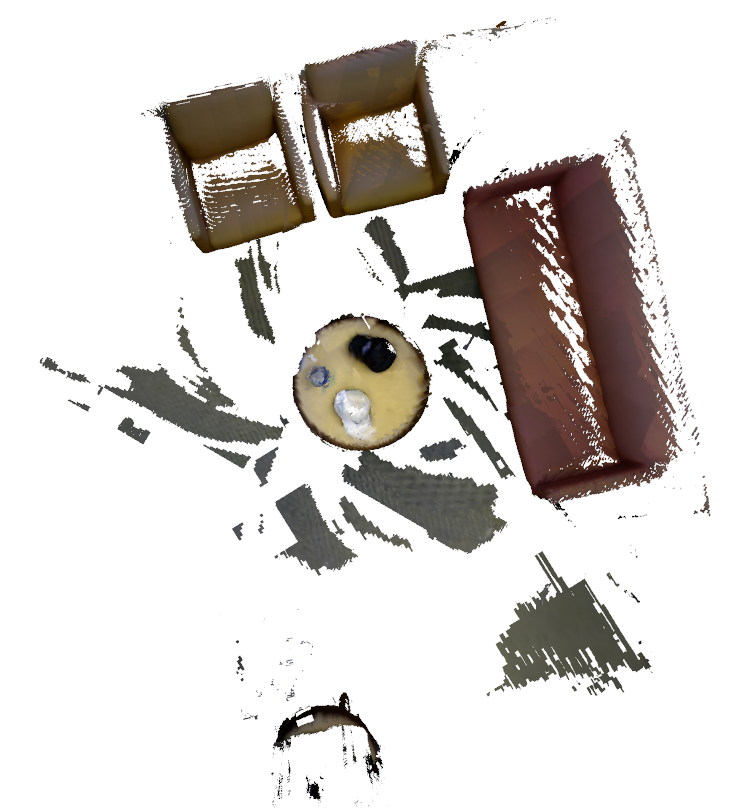
\includegraphics[align=c,width=0.5\linewidth]{figs/scene12.png}}
    \vspace{-2mm}
    \caption{Reconstructed small indoor scene \emph{RGB-D Scene 12}. We first show an example input \textit{RGB} frame followed by a top-down view of the reconstruction from \textit{MaskFusion}. This is followed by result from our pipeline. Note that in our reconstruction background walls and floor are filtered out. }
    \vspace*{-1em}
    \label{fig:rgbd_scene12}
\end{figure*}


\section{Quantitative results}

Table \ref{tab:ATE_RMSE} presents Absolute Trajectory Error (ATE) of four different methods compared with our system. Note in the table, that we \textit{bold} the best results of the object-based systems. We also provide results from geometric SLAM systems for comparison to present that our trajectory error is comparable to state of the art systems.

\begin{table*}[htbp]
\centering
\caption{Trajectory accuracy comparison on real world datasets (Absolute Trajectory Error in centimeters)}
\begin{tabular}{ |p{3cm}||p{2.2cm}|p{1.5cm}||p{2.2cm}| p{1.6cm} | p{1.5cm}|  }
 \hline
 Dataset & ElasticFusion & Open3D & MaskFusion & Fusion++ & Ours \\
 \hline
 Online & \checkmark &  & \checkmark & \checkmark & \checkmark \\
 \hline
 Object Models & & & \checkmark & \checkmark & \checkmark \\
 \hline \hline
RGBD Scenes - Scene 03 & 1.42 & 19.37 & 26.67 & - & \textbf{4.52}\\
\hline
RGBD Scenes - Scene 12 & 0.64 & 1.97 & 10.81 & - & \textbf{2.36}\\
\hline
RGBD Scenes - Scene 14 & 1.09 & 1.33 & 8.26 & - & \textbf{2.37}\\
\hline
fr1\_xyz & 6.33 & 6.64 & 8.68 & - & \textbf{7.50}\\
\hline
fr1\_desk & 2.70 & 5.73 & 24.05 & \textbf{4.9} & 5.82\\
\hline
fr1\_desk2 & 7.12 & 7.65 & 21.5 & 15.3 & \textbf{9.57}\\
\hline
fr1\_room & 22.06 & 5.65 & 52.4 & 23.5 & \textbf{21.7}\\
\hline
fr2\_xyz & 1.12 & 2.18 & 12.30 & \textbf{2.0} & 2.27\\
\hline
fr2\_desk & 7.61 & 4.72 & 163.6 & 11.4 & \textbf{9.94}\\
\hline
fr3\_long\_office & 2.23 & 3.54 & 140.8 & 10.8 & \textbf{9.68}\\
\hline
\end{tabular}
\label{tab:ATE_RMSE}
\end{table*}

In general, we achieve comparable results against the state-of-the-art surfel based online SLAM system \textit{ElasticFusion}~\cite{\whelanElasticFusionDenseSLAM2015} and volumetric offline reconstruction system \textit{Open3D}~\cite{zhouOpen3DModernLibrary2018}. In the meantime, our method outperforms object-based SLAM systems \textit{MaskFusion}~\cite{runzMaskFusionRealTimeRecognition2018}
t
and \textit{Fusion++}~\cite{mccormacFusionVolumetricObjectLevel2018} by a large margin. This improvement can be attributed to the use of semantic data association and scalable voxel grids. It must be noted that \textit{MaskFusion} requires 2 high end graphics cards to run it in online mode, therefore we ran it in offline mode, and stored all the detected object instances instead of manually selecting objects of interest for a fair comparison with our method. Additionally, we note that since Fusion++ is not open source, we obtain the results from the corresponding paper.

\begin{figure}[t!]
    \centering
    \subfloat[\label{sfig:obj_loop_closure_a}]{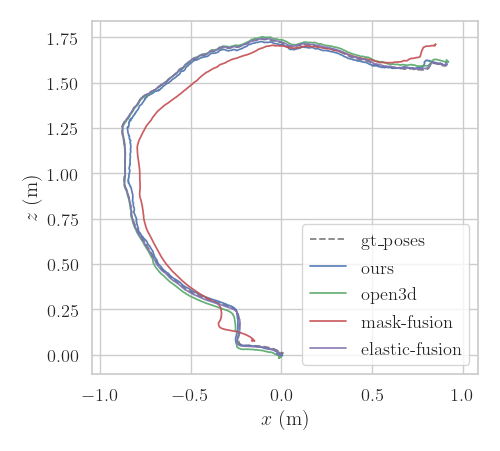
\includegraphics[width=0.5\linewidth]{figs/scene12-ape.png}}
    \subfloat[\label{sfig:obj_loop_closure_b}]{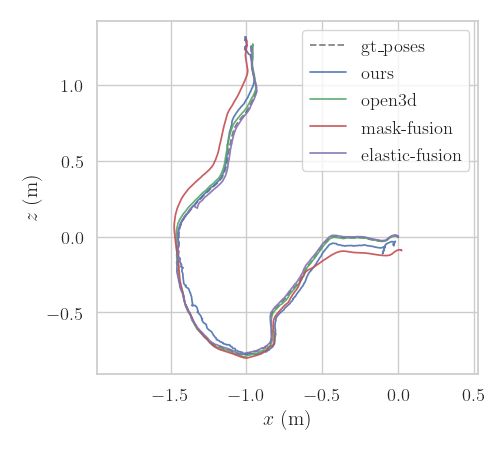
\includegraphics[width=0.5\linewidth]{figs/scene14-ape.png}}
    \caption{Comparison of trajectories between our pipeline and baselines with ground truth. (a) shows \emph{rgbd-scenes-v12} and (b) shows \emph{rgbd-scenes-v14} sequences. }
    \vspace*{-1em}
    \label{fig:rgbd_scenes-ape}
\end{figure}

For small scenes in the \textit{RGB-D scenes V2 dataset}, we achieve consistently high accuracy with ATE below $5cm$ for all scenes. Figure~\ref{fig:rgbd_scenes-ape} shows detailed trajectory visualizations.

For larger scenes, although noisy semantic segmentations affect masks and introduce noise for frame-to-model odometry, compositional rendering still ensures reliable tracking. Trajectory comparisons are provided in Figure~\ref{fig:fr3_household-ape}.


\begin{figure}[t!]
    \centering
    \subfloat[]{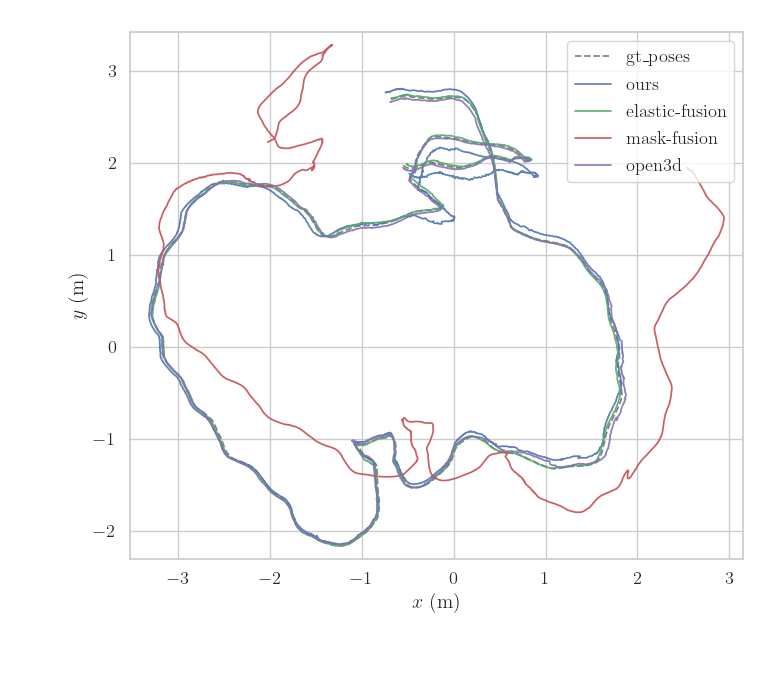
\includegraphics[width=0.5\linewidth]{figs/fr3_household-ape.png}}
    \subfloat[]{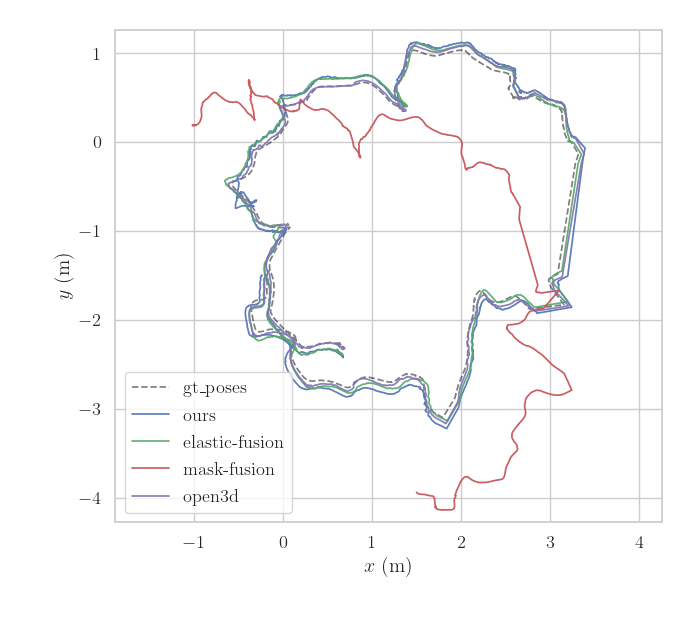
\includegraphics[width=0.5\linewidth]{figs/fr2_desk-ape.png}}
    \caption{Trajectory comparisons on the TUM-RGBD dataset (a) \emph{fr3\_long\_office\_household} and (b) \emph{fr2\_desk} sequences showing that even in the absence of explicit loop closures, our system maintains comparable accuracy.}
    \vspace*{-1em}
    \label{fig:fr3_household-ape}
\end{figure}
\section{Runtime analysis}

For runtime evaluation of our system we limit the number of initialized objects in the scene to 10 to ensure (close to) online performance on the aforementioned scenes. Processing each frame in the absence of any objects i.e., only background tracking takes about 200ms per frame. The largest computational bottleneck and time consuming operation is the rendering step, and while there are multiple rendering operations required (for instance, during object association), we render the objects and background only once per frame, and reuse the renders. We observe that each object takes on average about 45ms to render. In the presence of about 5-8 objects in the scene, the time taken per frame increases to about 450ms (200ms for background + 250ms for object renders) per frame. In comparison, we observed in our tests that \textit{MaskFusion} runs at lower than 1FPS with one graphics card and suffers from random crashes in online mode. \textit{Fusion++} reports its results with pre-computed segmentation masks. Our method runs seamlessly on a single GPU. A detailed runtime analysis is given in Table~\ref{tab:runtime}.

\begin{table}[ht]
    \centering
    \caption{Runtime breakdown component-wise for our pipeline}
    \resizebox{0.995\linewidth}{!}{
    \begin{tabular}{|c|c|c|c|c|c}
        \hline
        Component & Tracking & Segmentation & Association & Rendering\\
        \hline
         Time (ms) & 13 & 250 & 15 & 45 per object\\
        \hline
    \end{tabular}
    }
    \label{tab:runtime}
\end{table}
